\documentclass[12pt, oneside, titlepage]{article}   	% use "amsart" instead of "article" for AMSLaTeX format

\usepackage{graphicx}
\graphicspath{ {\string} }
\usepackage{subcaption}

\usepackage{tabularx}   


%%%%%%%%%%%%%%%%%%%%%%%%%%%%%%%%%%%%%%%%%%%%%%%%%%%%
% set up packages
%%%%%%%%%%%%%%%%%%%%%%%%%%%%%%%%%%%%%%%%%%%%%%%%%%%%
\usepackage{geometry}                
\usepackage{textcomp}                
\usepackage{amsmath}                
\usepackage{graphicx}                
\usepackage{amssymb}                
\usepackage{fancyhdr}                
\usepackage{subcaption}                
\usepackage{bm}                
\usepackage{lineno}
% package for comments
\usepackage{soul}
\sethlcolor{lightgray}

\usepackage{wrapfig}

\usepackage[usenames, dvipsnames]{color}

\usepackage[breaklinks=true]{hyperref}
\hypersetup{
    colorlinks=true,
    linkcolor=red,
    filecolor=orange,      
    urlcolor=red,
    citecolor=Violet,
}

\usepackage[superscript,noadjust]{cite} % puts dash in citations to abbreviate
\usepackage [autostyle, english = american]{csquotes} % sets US-style quotes

\usepackage{etoolbox} % block quotes

\usepackage{float}

\usepackage{pgf}
\usepackage{tikz}
\usepackage{eqnarray}

\usepackage{listings} % code blocks
\usepackage{setspace}

\usepackage{lscape}

\usepackage{natbib}
%\bibliographystyle{abbrvnat}
\setcitestyle{authoryear}

% Adds parentheses around year
%\setcitestyle{authoryear,open={(},close={)}}

%%%%%%%%%%%%%%%%%%%%%%%%%%%%%%%%%%%%%%%%%%%%%%%%%%%%
% call packages
%%%%%%%%%%%%%%%%%%%%%%%%%%%%%%%%%%%%%%%%%%%%%%%%%%%%	
\geometry{letterpaper, marginparwidth=60pt} % sets up geometry              		
\linenumbers % adds line numbers 
\MakeOuterQuote{"} % sets quote style
\doublespacing % setspace

%%%%%%%%%%%%%%%%%%%%%%%%%%%%%%%%%%%%%%%%%%%%%%%%%%%%
% patches with etoolbox 
%%%%%%%%%%%%%%%%%%%%%%%%%%%%%%%%%%%%%%%%%%%%%%%%%%%%	
% block quotes
\AtBeginEnvironment{quote}{\small}

% linenumbers
\makeatletter
\patchcmd{\@startsection}{\@ifstar}{\nolinenumbers\@ifstar}{}{}
\patchcmd{\@xsect}{\ignorespaces}{\linenumbers\ignorespaces}{}{}
\makeatother

%%%%%%%%%%%%%%%%%%%%%%%%%%%%%%%%%%%%%%%%%%%%%%%%%%%%
% tikzlibrary modifications
%%%%%%%%%%%%%%%%%%%%%%%%%%%%%%%%%%%%%%%%%%%%%%%%%%%%	
\usetikzlibrary{fit}
\usetikzlibrary{positioning}
\usetikzlibrary{arrows}
\usetikzlibrary{automata}

%%%%%%%%%%%%%%%%%%%%%%%%%%%%%%%%%%%%%%%%%%%%%%%%%%%%
% page formatting; exact 1 in margins
%%%%%%%%%%%%%%%%%%%%%%%%%%%%%%%%%%%%%%%%%%%%%%%%%%%%
\pagestyle{plain}                                                     

\setlength{\textwidth}{6.5in}    
\setlength{\oddsidemargin}{0in}
\setlength{\evensidemargin}{0in}
\setlength{\textheight}{8.5in}
\setlength{\topmargin}{0in}
\setlength{\headheight}{0in}
\setlength{\headsep}{0in}
\setlength{\footskip}{.5in}

%%%%%%%%%%%%%%%%%%%%%%%%%%%%%%%%%%%%%%%%%%%%%%%%%%%%
% defining code blocks using listings package
%%%%%%%%%%%%%%%%%%%%%%%%%%%%%%%%%%%%%%%%%%%%%%%%%%%%

\definecolor{dkgreen}{rgb}{0,0.6,0}
\definecolor{gray}{rgb}{0.5,0.5,0.5}
\definecolor{mauve}{rgb}{0.58,0,0.82}

\lstset{frame=tb,
  language=R,
  aboveskip=3mm,
  belowskip=3mm,
  showstringspaces=false,
  columns=flexible,
  basicstyle={\small\ttfamily},
  numbers=none,
  numberstyle=\tiny\color{gray},
 % keywordstyle=\color{blue},
  commentstyle=\color{dkgreen},
  stringstyle=\color{mauve},
  breaklines=true,
  breakatwhitespace=true,
  tabsize=3,
  otherkeywords={0,1,2,3,4,5,6,7,8,9},
  deletekeywords={data,frame,length,as,character,dunif,ps},
}

%%%%%%%%%%%%%%%%%%%%%%%%%%%%%%%%%%%%%%%%%%%%%%%%%%%%
%%%%%%%%%%%%%%%%%%%%%%%%%%%%%%%%%%%%%%%%%%%%%%%%%%%%
% begin document
%%%%%%%%%%%%%%%%%%%%%%%%%%%%%%%%%%%%%%%%%%%%%%%%%%%%
%%%%%%%%%%%%%%%%%%%%%%%%%%%%%%%%%%%%%%%%%%%%%%%%%%%%

\begin{document}

%%%%%%%%%%%%%%%%%%%%%%%%%%%%%%%%%%%%%%%%%%%%%%%%%%%%
% TITLE PAGE
%%%%%%%%%%%%%%%%%%%%%%%%%%%%%%%%%%%%%%%%%%%%%%%%%%%%
\begin{titlepage}
   \begin{center}
       \vspace*{1cm}
 
       \textbf{\hl{[Working title]}: Intraspecific variation in range-wide seed bank dynamics is not consistent with density-independent model of bet hedging}
 
       \vspace{1.5cm}
 
       Gregor-Fausto Siegmund and Monica Geber
 
   	Last updated: \today
	
	\iffalse
	\section*{Writing list}
	
	\begin{enumerate}
	
	\item Read Cohen \& Ellner to identify the role of complete reproductive failure in the original models for the evolution of bet hedging
	\item Write description of modeling for the seed bag experiment
	\item Write about strong and weaker test of the hypothesis (partial pooling, no partial pooling) 
	\item Write paragraph about history of studies of bet hedging via seed bank, with emphasis on how this study addresses this question at an intraspecific level. Lower level of variation in intraspecific germination fraction. (\hyperlink{bet-hedging-history}{link})
	\item Write models for belowground vital rates
	\item Revise description for density-independent model for germination probability
	\item Write and implement model checking process
	
	\end{enumerate}
	\fi
 
   \end{center}
\end{titlepage}
%

%%%%%%%%%%%%%%%%%%%%%%%%%%%%%%%%%%%%%%%%%%%%%%%%%%%%
% INTRODUCTION
%%%%%%%%%%%%%%%%%%%%%%%%%%%%%%%%%%%%%%%%%%%%%%%%%%%%
\section*{Introduction}

%General introduction to seed banks/dormancy -- Clarkia as a case where seed banks have been posited to be important -- bet hedging theory and predictions -- review of tests of bet hedging in plants -- what we did

Seed banks can buffer plant populations against environmental change and stochasticity (\cite{eager2014,paniw2017}), increase effective population size (\cite{nunney2002,waples2006}), and maintain genetic diversity (\cite{mccue1998b}). Dormancy can affect the outcome of evolution (\cite{ritland1983,heinrich2018}). Theory thus suggests that seed banks have ecological and evolutionary consequences (\cite{evans2005}). 

What drives the evolution of delayed germination? The \hl{theory} developed by \cite{cohen1966} frames the problem in the following terms. What is the optimal germination fraction for a given level of interannual variation in fitness and seed survivorship? These models make it clear that the germination fraction that maximizes long-term population growth rate is a function of the distribution of fitness (characterized by the variation in fitness), the fitness values, and the rate of seed survivorship. For a given mean fitness, increasing the variance in fitness decreases the optimal germination fraction. Increasing seed survivorship decreases the optimal germination fraction, and the degree to which it does so depends on the probability of a 'good year'. Specifically, as the probability of a high-fitness year decreases, the optimal germination fraction decreases. Bet hedging should evolve to maximize the long-term geometric population growth rate (as compared to the arithmetic population growth rate) (\cite{cohen1966,cohen1968,ellner1985,ellner1985a}). 

%Cohen (1966) emphasizes the role of particularly bad years. This is highlighted by the inequality in equation (12), which states that for the optimal germination strategy to be bet hedging, it is sufficient that the harmonic mean is less than the survival probability of seeds that do not germinate. The minimum fitness has a strong impact on the harmonic mean of fitness (see definition of harmonic mean on Wikipedia), and a single year of very low fitness would tend to make the harmonic mean small. In particular, the harmonic mean is 0 when any of its values is 0. The probability of complete reproductive failure is thus particularly important. Years with no seedling survival in the plots or no germination are those in which fitness would be zero; there are only 4/20 populations in which this does not happen. We fit two types of models to the aboveground data; one with partial pooling and one with no pooling. The first was an attempt to correct for sampling variation; the latter an attempt to estimate per-capita reproductive success as-is, providing a more extreme estimate of interannual variation but one that reflects the combined effect of sampling variation and true variation.

%\hl{Revisit theory to see particular role of complete reproductive failure versus low fitness years more generally.}

%In paragraph on \hl{theory}, discuss density-independent models \cite{cohen1966,cohen1968}, density-dependent models \cite{ellner1985,ellner1985a}, predictive germination \cite{cohen1967}, and unstructured versus structured models \cite{easterling2000} (\hl{Tuljaparkur 1993, Valleriani and Tielborger 2006}).

%To empirically test this theory, "a density-independent model can be used to check quantitatively the optimality (or evolutionary stability) of a life history trait in a real population, because the density effects are manifested in the measured vital rates" and "to check if a species germination fraction is optimal, one would estimate seed survivorship and the probability distribution of per capita seed yield. From these, the DI model predicts an "optimal" germination fraction, which can be compared with the actual germination fraction." \cite{ellner1985a}.

%Several studies have examined intraspecific variation in seed dormancy \cite{hacker1984,hacker1989,philippi1993a,clauss2000}. The main set of papers I've included are ones that look at variation in germination among Sonoran Desert annuals (\cite{venable2007,gremer2014,gremer2016}). The table lists predictions made by different models. I think examining the following relationships would be good starting points: The correlation between variance in fitness (seeds/seedling) and germination fraction should be negative -- this is true under the density-independent and -dependent model. The correlation between seed survivorship and germination fraction should be negative under both a density-independent and -dependent model but the limit as survivorship approaches 1 differs. Finally, the correlation between mean seed yield and germination fraction will be positive if fitness is density-independent but is not necessarily positive if fitness is density-dependent.

%\hypertarget{bet-hedging-history}{\hl{Paragraph about the history of empirical studies of bet hedging.}}

Population vital rates are known to exhibit intraspecific variation across \textit{Clarkia xantiana}'s geographic range, including age-specific germination and seed survival (\cite{eckhart2011}). In a study of \textit{C. xantiana} population dynamics that identified a decline of long-term stochastic population growth rate from west to east across the range, \cite{eckhart2011} inferred a decrease in survival through winter ($s_1$) and an increase in germination rate ($g_1$) of first-year seeds from west to east. Although, \hl{Lewis 1962} suggested that \textit{Clarkia} populations undergo local extinctions and lack a long-lived seed bank, observations of 20 populations across the range are not consistent with that hypothesis (Figure~\ref{fig:zero-fitness}). Demographic observations \cite{eckhart2011} and transplant experiments demonstrate that fitness can exhibit dramatic interannual variation (e.g. 30-fold between a wet and dry year in \hl{Geber and Eckhart 2005}). 

Seed dormancy and persistence in the soil seed bank may be a bet-hedging strategy that is favored by environmental uncertainty. If this is the case in \textit{C. xantiana}, we might expect increased seed survival and decreased germination probabilities in populations with more variability in per-capita reproductive success. However, broad geographic patterns in rainfall variability and life history are not consistent with this cursory explanation since variation in rainfall increases from west to east, and germination probability also increases \cite{eckhart2011}. We thus sought to understand intraspecific variation in \textit{C. xantiana} seed vital rates in the context of broader life history patterns. 

Bet hedging should evolve to maximize the long-term geometric population growth rate (as compared to the arithmetic population growth rate) (\cite{cohen1966,cohen1968,ellner1985,ellner1985a}). Seed banks are more likely to be selected in populations which experience higher levels of interannual variation in per-capita reproductive success. To investigate this empirical relationship, we estimate the correlation between germination and seed survival, and between germination variance in per-capita reproductive success. We also examined whether observed levels of germination are consistent with germination levels predicted by a density-independent model of bet hedging. 

% the correlation between interannual variation in per-capita reproductive success and the proportion of seeds that germinate in the winter immediately following seed production. Based on bet hedging models, we predict that germination is negatively correlated with interannual variation in per-capita reproductive success. %[What is the relationship between interannual variation in fitness and dormancy? This is a question about whether fitness variation and dormancy are positively correlated as expected ? this is what selects for bet hedging.]

 %A previous study with \textit{Clarkia xantiana} suggests that the soil seed bank is important for population dynamics in \textit{Clarkia xantiana} . 


%A separate set of seed burial experiments suggests that seeds of \textit{C. xantiana} can remain viable in the soil for at least 10 years (Moeller personal communication). In the study of \textit{C. xantiana} population dynamics that showed a decline of long-term stochastic population growth rate from west to east across the range, \cite{eckhart2011} inferred a decrease in survival through winter (s1) and an increase in germination rate (g1) of first-year seeds from west to east.



%Population growth rates determine species abundance and distribution, and are ultimately what limit persistence beyond range edges. Geographic patterns to vital rates have so far been studied to help understand the demography of geography. Seed banks are a strategy that annual plants may use to buffer against environmental variation and may be part of population persistence. I will begin by characterizing geographic variation in belowground vital rates. [What is the geographic pattern to variation in germination or seed survival?] [I think this question could be expanded to make clear predictions and/or address another aspect such as variation in time.]

%\hl{Eckhart et al. 2004} conducted a transplant experiment in two years in which seed set varied ten-fold. There are additional studies that did elimination experiments (with other species of Clarkia) and suggested limited role/role for seed bank because plants did or did not come up with following year. 

% In \hl{13 years} of data on 20 populations across the species range, we observed high seedling mortality and/or low germination in at least one year in all but four populations. Although most populations had at least some flowering plants in most years, there were also four populations in which no flowering plants were observed in the entire population. None of these populations, however, went extinct during the period of the study. Seeds can remain viable in the field and laboratory for at least 5 years, contrary to previous suggestions that seeds are unlikely to persist past a few years (\hl{Lewis 1962}). 


%\hl{See also the comments in Lewis 1953 on lifespan of seeds, absence of dormancy, and cued germination. Lewis 1963 Presidential address at SSE on catastrophic selection is also relevant. Discusses extinction and possible absence of a seed bank in populations of Clarkia species. Specifically mentions a population in the upper Kern Valley that had both whites and pinks; the pinks went extinct during a drought year while the whites maintained their population size. This work was followed up by others on different species in Clarkia genus. I think its important to consider the possibility that C. xantiana being studied in 1963 was a xantiana/parviflora ssp. which may have different dynamics than the outcrossing xantiana/xantiana. Furthermore: the upper parts of the range have the highest rates of germination which may also trade off with low survival. It would be interesting to put that observation in the range-wide context!} 

%\hl{Knies et al. 2004} studied 2 C. xantiana populations; seeds of outcrosser are heavier than selfers. Identify heavier seeds (~.1 mg heavier at SC than WH population). Seeds from both populations were bullet-shaped but differ in shape of exotesta cells; WH cells are gourd shaped, SC shapes are even width and spherical. Seed size/number trade-off: smaller size for dispersal; greater mass increases germination probability. Smaller seed size also facilitates seed integration into soil seed bank. Small seed size is also correlated with a persistent seed bank (Thompson et al. 1993). Larger seeds may germinate under more conditions and perhaps have smaller seed bank.

%\hl{Moeller et al. 2011} population genetic study. 

%\hl{Eckhart and Geber 1999} identify more populations than those of Lewis, populations that they have since monitored intensively. 

%\hl{Price et al. 1985} followed a population for 2 years, did an elimination experiment. determined a dormant seed bank.  \hl{Snow 1960} reports eliminating plants and not observing plants the following year. 

%\hl{Geber and Eckhart 2005} observed a 30-fold difference in lifetime fitness [calculated as number of germinants times survival, flower number, fruit set and seed set] between two transplant years (one wet, one dry). Fitness was very low in the dry year of the study (0.02-0.03 seeds per seed planted). They observed a 2-4 fold difference between years in germination, seedling survival, and flower number. They did not observe a difference in fruit or seed set. Western populations showed evidence of regional adaptation: survival and flower number. Germination declined from the western to eastern transplant sites [in contrast to what we observe here?] Germination is consistently higher in subspecies xantiana than parviflora. From west to east, rainfall declines and becomes more variable. Low survivorship is the product of end-of-season drought, small mammal herbivory (\hl{Geber and Eckhart 2005, Benning et al. 2019}), competition by higher vegetation cover of grasses (survivorship increases with plant size), fungal rust infection. Plants from western populations are larger. Note that the transplant experiments took place on igneous soils, and later work by Vince has shown that soil type is important. 

%\hl{Eckhart et al. 2010 IJPS}: geographic patterns in precipitation, decline from west to east, mirrored geographic pattern in midday water potential (reduced performance). Metasedimentary soils were more resistant and finer. Soil characteristic curves indicated that metasedimentary soils can hold more water but that it becomes unavailable to plants at higher water contents. Higher water potential on steeper, eroding slopes; this soil was softer and coarser. Decline in soil water potential (more negative) decreases plant size and fruit number. However, soil water potential is unrelated to seedling survival in the study years. Metasedimentary rocks may compound effect of decline in precipitation. Metasedimentary rocks may hold more water but it may be more available to plants in igneous soils. 

%Bet hedging should evolve to maximize the long-term geometric population growth rate (as compared to the arithmetic population growth rate) (\cite{cohen1966,cohen1968,ellner1985,ellner1985a}). Seed banks are more likely to be selected in populations which experience higher levels of interannual variation in per-capita reproductive success. To investigate this empirical relationship, I will estimate the correlation between interannual variation in per-capita reproductive success and the proportion of seeds that germinate in the winter immediately following seed production. I predict that germination is negatively correlated with interannual variation in per-capita reproductive success. [What is the relationship between interannual variation in fitness and dormancy? This is a question about whether fitness variation and dormancy are positively correlated as expected ? this is what selects for bet hedging.]

%Seed dormancy and persistence in the soil seed bank may be a bet-hedging strategy that is favored by environmental uncertainty. If this is the case in \textit{C. xantiana}, I think we might expect increased seed survival and decreased germination at the eastern range edge (precipitation is more variable at eastern populations in winter and spring). This seems to be opposite of what was observed in the previous study ? though I could also be misinterpreting this. This is could be one reason to revisit this question with a new analysis. 


%Why using the Clarkia system? We expect to see differences among populations in either seed survivorship or variance in fitness. In the study of \textit{C. xantiana} population dynamics that showed a decline of long-term stochastic population growth rate from west to east across the range, Eckhart et al. 2011 inferred a decrease in survival through winter (s1) and an increase in germination rate (g1) of first-year seeds from west to east. [need to be clear about this] also know that the environment changes across the range; that will affect the mean fitness

%I expect bet hedging stages to be sensitive to variation in an environmental cue. For something to be an adaptive strategy, it should respond to variation in the environment to capitalize on good years such as ones with high precipitation. To investigate the sensitivity of vital rates to the environment, I estimate the slope of the relationship between environmental cues and vital rates at individual sites using a random coefficients model that estimates covariation between intercepts and slopes. I predict that I will estimate variation both in the intercept and slope for populations, and that variation in the modeled cue [to be determined] will be positively related to the estimated slope. [What is the relationship between dormancy and environmental cues? This is a question about whether we can make any inferences about the mechanism responsible for bet hedging in this system.]

\iffalse
\singlespace
\begin{center}
\captionof{table}{Models for germination delays: references and predictions } \label{tab:title} 
\resizebox{\textwidth}{!}{
\begin{tabular}{ |p{2.5cm}|p{4cm}|p{4cm}|p{4cm}|p{4cm}|  }
 \hline
  & Density-independent fitness & Density-dependent fitness & Predictive germination & Structured model \\
 \hline
 Key theory references   & \cite{cohen1966,cohen1968}    & \cite{ellner1985,ellner1985a} &   \cite{cohen1967} & \hl{Tuljapurkar and Istock 1997} \cite{easterling2000} \hl{Valleriani and Tielborger 2006} \\
 \hline
 Key empirical tests & \cite{venable2007}  & \cite{gremer2014}   & \cite{gremer2016} & ... \\
 \hline
 Mean of \newline seed yield    & increase in $\bar{Y}$ increases $G$* & increase in $\bar{K}$ can increase or decrease $\hat{G}$  &  \dots & \dots \\
 \hline
 CV of \newline seed yield & increasing $\rho_Y$ decreases $G$* & increasing $\rho_K$ or $\rho_C$ decreases $\hat{G}$ &  \dots  & \dots \\
 \hline
 Seed \newline survivorship & increasing $s$ decreases $G$*; limit near $s=1$ is p & increasing $s$ decreases $\hat{G}$; limit near $s=1$ is 0  & \dots  & \dots \\
 \hline
 %Frequency of good years & higher frequency of good years increases $G$*  & high frequency of good or bad years decreases $\hat{G}$   & \dots & \dots \\
%\dots & \dots & \dots  & years with high G correspond to years with high Y & \dots \\
\end{tabular}}
\end{center}
\doublespace
\fi
%%%%%%%%%%%%%%%%%%%%%%%%%%%%%%%%%%%%%%%%%%%%%%%%%%%%
% METHODS
%%%%%%%%%%%%%%%%%%%%%%%%%%%%%%%%%%%%%%%%%%%%%%%%%%%%
\section{Methods}

\subsection{Clarkia life history}

\textit{Clarkia xantiana} is a winter annual that germinates with late fall and winter rains. In our study region, the Kern Valley in the southern Sierra Nevada Mountains, historically happens between October and late February or early March. Seedlings grow throughout the winter and spring, and surviving plants flower in late spring and early summer, April into early July. Pollinated fruits set seed in the early summer, June to July. Seeds of \textit{C. xantiana} are produced in early summer, with fruits that dry out and gradually split open. Most seeds appear to be shed from fruits within 3-4 months after production, but can remain on the plant for up to a year. Seeds are small ($<1$ mm in width) and have no structures to aid in aerial dispersal. 

\iffalse
\begin{wrapfigure}[]{r}{0.5\textwidth}
       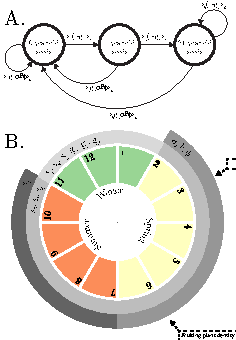
\includegraphics[scale=1.9]{../manuscript/figures/model-figure.pdf}  
        \caption{ Diagram representations of Clarkia life cycle. }
        \label{fig:life-cycle}
\end{wrapfigure}
\fi

We represent the \textit{Clarkia xantiana} as a life cycle graph (Figure \ref{fig:life-cycle}A) that describes transitions from October of year $t$ to October of year $t+1$ in terms of underlying vital rates. The census period occurs when the entire population is seeds, and corresponds to the time at which seed bags are placed into the field (\hl{see below}). Seeds are grouped into three stages: age 0 seeds, which were produced in the current year; age 1 seeds, which were produced in the previous year; age 2+ seeds, which were produced two or more years ago. Persistence of seeds in the seed bank is represented by transitions from younger to older seeds. Production of new seeds is captured by transition to the age 0 seed state. 

Transitions in the life cycle graph are the product of age-specific seed survival and germination, and aboveground seedling survival to fruiting, fruit production, and seeds per fruit. Seed-related rates are represented separately for age 0, 1, and 2+ seeds. Germination for each age class is given as $g_1$, $g_2$, and $g_3$, respectively. Seed survival from seed production to the first October is given as $s_0$, and survival from October to February is given as $s_1$, $s_3$, and $s_5$ for age 0, 1, and 2+ seeds, respectively. Survival from February to October is given as $s_2$, $s_4$, and $s_6$ for age 0, 1, and 2+ seeds, respectively. We assume that vital rates remain unchanged after age 2. We also we assume that all plants experience the same vital rates upon germination seed age at germination does not affect seedling survival to fruiting ($\sigma$), fruits per plant ($F$), or seeds per fruit ($\phi$).

The life cycle graph (Figure \ref{fig:life-cycle}A) corresponds to the annual projection matrix
%
\begin{gather}
\bm{A} = 
\begin{bmatrix} 
s_1 g_1 \sigma F \phi s_0 & s_3 g_2 \sigma F \phi s_0 & s_5 g_3 \sigma F \phi s_0 \\
s_1 (1-g_1) s_2 & 0 & 0 \\
0 & s_3 (1-g_2) s_4  & s_5 (1-g_3) s_6  \\
\end{bmatrix}
\label{eq:projection-matrix}
\end{gather} 
%
that summarizes transitions between stages. 

\subsection{Creating the dataset}

We used field experiments and surveys to assemble observations of below- and above-ground demography for 20 populations of \textit{Clarkia xantiana} (Table \ref{tab:datasets}). Specifically, we used experiments to estimate transitions in the seed bank and surveys to estimate components of per-capita reproductive success. These demographic data have previously been used to test hypotheses about the geography of demography (\hl{Eckhart et al. 2011}) and species distributions (\hl{Pironon et al. 2018}). Here, we sought to obtain population-level estimates of germination and seed survival, and yearly estimates of per-capita reproductive success.

To estimate transitions in the seed bank, we used observations from a seed bag burial experiment conducted in all populations from 2006-2009 (Figure \ref{fig:seed-bag-experiments}). The experiment has been previously described in \hl{Eckhart et al. 2011} and we reanalyze the data here. \hl{Geber and collaborators} buried seeds in bags and unearthed 1, 2, or 3 years after being buried to count seedlings and intact, viable seeds. The experiment was repeated in 3 consecutive years and ended in 2009. We thus have 3 sets of observations associated with 1 year old seeds, 2 sets of observations associated with 2 year old seeds, and 1 set of observations associated with 3 year old seeds. We use data from the experiment to estimate age-specific germination and seed survival (\hl{see Joint model for seed vital rates}) but note that we test predictions of bet-hedging theory that are based on an unstructured seed bank and use only the relevant subset of transitions in our analysis (\hl{see Computing vital rates}).

To estimate per-capita reproductive success, we combine censuses of seedlings and fruiting plants, surveys of fruits per plant, and lab counts of seeds per fruit. To assess the survival of seedlings to fruiting plants, we counted seedlings and fruiting plants in 30 0.5 m$^2$ permanent plots from 2006--\hl{2018} (\hl{Eckhart et al. 2011}). To assess seed production by plants that survive to reproduction, we counted fruits per plant on individual plants in permanent plots, and on additional haphazardly chosen plants throughout the population. We then attempted to obtain 20-30 fruits per population, which we used to count seeds per fruit (\hl{Eckhart2011}). 

\begin{singlespace*}...
\captionof{table}{ Summary of data sets used to estimate parameters. } \label{tab:datasets} 
\begin{center}
%\documentclass[varwidth=\maxdimen,border=1pt]{standalone}
%                 
%\usepackage{bm}   
%\usepackage{tabularx}   
%
%\usepackage{caption}          
% \captionsetup[table]{labelfont=sc}
%
%\usepackage{amsmath}                      
%\usepackage{amssymb}      
%
%
%%%%%%%%%%%%%%%%%%%%%%%%%%%%%%%%%%%%%%%%%%%%%%%%%%%%%
%%%%%%%%%%%%%%%%%%%%%%%%%%%%%%%%%%%%%%%%%%%%%%%%%%%%%
%% begin document
%%%%%%%%%%%%%%%%%%%%%%%%%%%%%%%%%%%%%%%%%%%%%%%%%%%%%
%%%%%%%%%%%%%%%%%%%%%%%%%%%%%%%%%%%%%%%%%%%%%%%%%%%%%
%
%\begin{document}

%%%%%%%%%%%%%%%%%%%%%%%%%%%%%%%%%%
% DATASETS
%%%%%%%%%%%%%%%%%%%%%%%%%%%%%%%%%%

%\captionof{table}{ Summary of data sets used to estimate parameters. } \label{tab:title1} 
  \begin{tabularx}{\linewidth}{ l l c c } 
 \hline
 \hline
\multicolumn{1}{ c }{ Parameter data } & 
\multicolumn{1}{ c }{ Description } & 
\multicolumn{1}{ c }{ Data set }  & 
\multicolumn{1}{ c }{ Time span } \\
 \hline
 % seed bag burial experiment
 \textsc{Seed vital rates} & --- & --- & --- \\ 
 Seed survival and germination & Seed bag burial & $\bm{\mathrm{Y}}_1$ & 2006-2009  \\ 
 Seed viability & Viability trials & $\bm{\mathrm{Y}}_2$ & 2006-2009 \\ 
 Seed survival and germination & Seed pots & $\bm{\mathrm{Y}}_3$ & 2013-2019  \\ 
 \textsc{Seedling survival} & --- & --- & --- \\ 
 Seedling survival to fruiting & Field surveys & $\bm{\mathrm{Y}}_4$ & 2006-2019 \\ 
 \textsc{Fruits per plant} & --- & --- & --- \\ 
 Total fruit equivalents per plant & Field surveys & $\bm{\mathrm{Y}}_5$ & 2006-2012 \\ 
 Undamaged and damaged fruits per plant & Field surveys & $\bm{\mathrm{Y}}_6$ & 2013-2019 \\ 
 Total fruit equivalents per plant & Extra plots & $\bm{\mathrm{Y}}_7$ & 2006-2012 \\ 
 Undamaged and damaged fruits per plant & Extra plots & $\bm{\mathrm{Y}}_8$ & 2013-2019 \\ 
 \textsc{Seeds per fruit} & --- & --- & --- \\ 
  Seeds per undamaged fruit & Lab counts & $\bm{\mathrm{Y}}_9$ & 2006-2019 \\ 
  Seeds per damaged fruit & Lab counts & $\bm{\mathrm{Y}}_{10}$ & 2013-2019 \\   
  \hline
\end{tabularx} 
%\end{document}
\end{center}
\end{singlespace*} 

\iffalse
\begin{figure}[!h]
       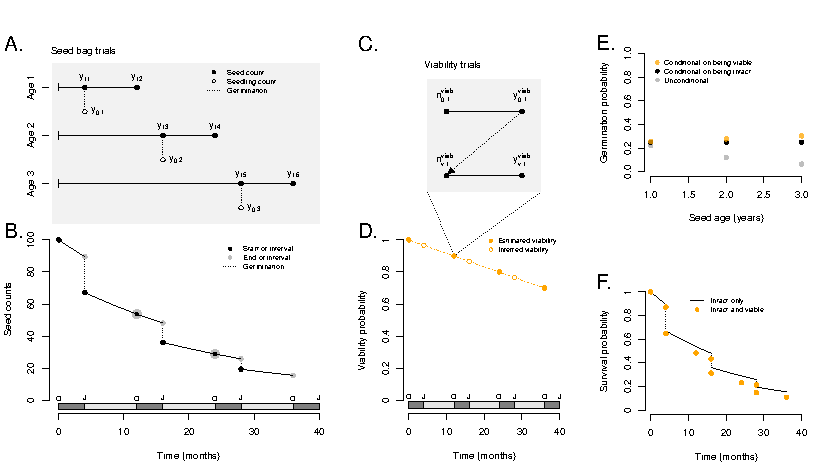
\includegraphics[width=\textwidth]{../manuscript/figures/seed-bag-figure.pdf}  
    \caption{ Summary of the seed bag burial experiments and viability trials. \hl{Figure will be labeled as (A-B: seed bag trials, C-D: viability trials, E-F: germination probability and survival probability. Add month markers to the y-axis in panels B, D, F}. (A) The gray panel contains a graphical representation of the seed bag trials. Seeds were buried at the start of each experiment (100 seeds in month 0). Seed bags were unearthed and intact seeds ($y_{\cdot \cdot}$) and germinants ($y_{\mathrm{g},\cdot}$ counted. The graph below the panel shows a hypothetical survival function associated with persistence of seeds in the soil seed bank. (B) The gray panel contains a graphical representation of the viability trials. Seeds were tested in two rounds; germination trials were performed and then some or all of the ungerminated seeds were tested for viability. The graph below the panel shows hypothetical data from a series of viability trials and the interpolated, inferred viabilities at times when viability was unobserved. (C) Age-specific germination probably is summarized in three ways. (D) The graph shows the survival function for persistence of seeds in the soil seed bank (black line) and the estimated discrete survival probabilities for persistence and viability of seeds (orange points). }
 \label{fig:seed-bag-experiments}
\end{figure}
\fi

\subsection{Model}

We use observational and experimental data from 20 populations of \textit{Clarkia xantiana} to estimate transition probabilities across the life cycle. We fit multilevel models to obtain population-specific estimates for belowground vital rates, and year- and population-specific estimates for aboveground vital rates. Because we were interested in describing the life histories of individual populations, we built separate models for each population. Our general approach applies a common model structure to partially pool observations from each population. 

We first explicitly describe our formulation in terms linear mixed models before defining the joint posterior (\hl{Evans et al. 2010, Ogle and Barber 2020}). We assume that the latent mean of observations in year $j$ at a population $k$, $\theta_{jk}$, is drawn from a normal distribution with mean $\theta_{0,k}$ and variance $\sigma^2_j$.

\begin{align}
  \begin{split}
  \theta_{jk} &  = \theta_{0,k} +\epsilon_{(jk)}.
  \end{split}
\end{align}

Our model includes a population-level intercept $\theta_{0,k}$ and random effects $\epsilon_{(jk)}$. The random effects can be written as  $\epsilon_{(jk)}\sim N(0, \varsigma^2)$. For the moment, we focus on describing the hierarchical structure of the model but note that we use link functions for transformation to parameters that are appropriate for the likelihoods we use to model different sets of observations (e.g. binomial for seed bag experiments; Poisson for counts of seed per fruit). We note that such a linear mixed effects model with random intercepts for years is one method commonly used to model interannual variation in demographic rates (\hl{e.g. Metcalf et al. 2015}). Using hierarchical centering, the same model is rewritten as 

\begin{align}
  \begin{split}
  \theta_{jk} &  = \alpha_{(jk)}.
  \end{split}
\end{align}

The mean $\theta_{jk}$, is now drawn from a normal distribution with mean $\alpha_{(jk)}$ and variance $\sigma^2_j$. We place a prior on $\alpha_{(jk)}$ such that $\alpha_{(jk)}\sim N(\theta_{0,k}, \varsigma^2)$. The expressions are related by $\alpha_{(jk)}=\theta_{0,k}+\epsilon_{(jk)}$. We thus draw year-level means from the population-level means. 

For a single population (ie. suppressing subscript $k$), we write the the posterior proportional to the joint distribution as

\begin{align}
  \begin{split}
  [ \theta_j , \theta_0 , \sigma_j^2 , \varsigma^2 | y_{ij} ] &  \propto [ y_{ij} | \theta_j , \sigma^2_j] [ \theta_j | \theta_0 , \varsigma^2 ] [ \theta_0 ] [ \sigma^2_j] [ \varsigma^2].
  \end{split}
\end{align}

\iffalse
\begin{wrapfigure}[]{r}{0.5\textwidth}
%\begin{figure}[!h]
       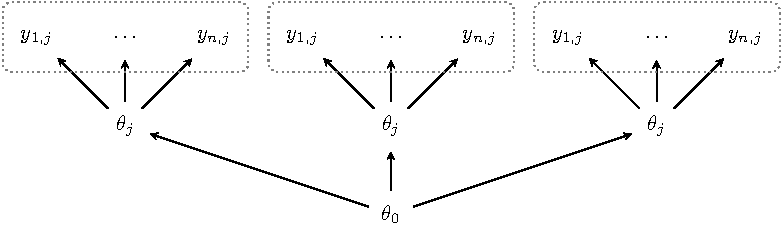
\includegraphics[scale=.65]{../manuscript/figures/dag-partialpool.pdf}  
    \caption{ Graph depicting the general structure for the hierarchical models, for one populatoin. Observations from each year, $y_{ij}$, are shown grouped and outlined by dotted lines. The observations are drawn from year-level parameters, $\theta_j$, which in turn are drawn from a population-level parameter, $\theta_0$. The graph omits variance terms. }
 \label{fig:hierarchical-dag}
%\end{figure}
\end{wrapfigure}
\fi

The distribution of the observations $y_{ij}$ is conditional on the year-specific parameters $\theta_j$ and $\sigma^2_j$. In turn, the year-specific parameter $\theta_j$ is conditional on the population-specific parameters $\theta_0$ and $ \varsigma^2$. We placed priors on all parameters found only on the right hand side of conditional statements ($\theta_0, \sigma^2_j, \varsigma^2$). In practice, we implemented this model by specifying the population- and year-levels of the model with normal distributions; for example, $[ \theta_j | \theta_0 , \varsigma^2 ]$ is $\theta_j \sim N(\theta_0, \varsigma^2)$. The model thus describes a structure in which years are nested within populations.

\subsection{Model statements, implementation, and fitting}

We include the expression for the posterior proportional to the joint distribution, and corresponding directed acyclic graphs, in \hl{Appendix: Joint Posterior}. Priors for all parameters are defined in \hl{Table Priors}. We applied the following principles for specifying priors: (1) we used weakly informative priors that avoided placing probability mass on biologically implausible values (\hl{Gelman; Lemoine; Wesner and Pomeranz}), (2) we placed positive, unbounded priors on variance components (\hl{REF}), (3) we conducted prior predictive checks to assess the scale of priors after parameter transformation (\hl{Hobbs and Hooten; Gabry; Wesner and Pomeranz}), and (4) we simulated prior predictive distributions to confirm that the joint likelihood generated data within the observed range (\hl{Gabry; Conn; Hobbs and Hooten}). We provide additional detail regarding our choice of priors in \hl{Appendix: Priors}. 

We prepared data for analysis using the tidyverse and tidybayes packages (\hl{CITE}) in R \hl{VERSION; CITE}. We wrote, fit all models, and estimated posterior distributions using JAGS \hl{VERSION} with rjags (\hl{Plummer 2016}). We randomly generated initial conditions for all parameters with a prior by drawing from the corresponding probability distribution in R before passing the initial values to rjags. We ran three chains for \hl{XX,000} iterations. The first \hl{XX,000} samples were discarded as burn-in and we sampled the following \hl{XX,000} iterations. \hl{We did not thin the chains (Elderd and Miller 2016)}.

We assessed convergence of the MCMC samples with visual inspection of trace plots, by calculating the Brooks-Gelman-Rubin diagnostic (R-hat), and by calculating the Heidelberg-Welch diagnostic (\hl{Elderd and Miller 2016}. The Gelman-Rubin diagnostic is used to assess convergence between chains and the Heidelberg-Welch for stationarity within chains. Trace plots for all chains, histograms of R-hat, and the percentage of chains that passed the HW test are shown in the appendix. 
 
To evaluate our model's fit to the data, we performed model checks that are described in full in \hl{Appendix: Model Checking}. We used our posterior distribution to simulate replicate datasets based on the parameters of our model. We compared samples from the simulated datasets to the real, observed datasets using both graphical, visual checks and by calculating Bayesian \textit{p}-values for test statistics calculated for the observed and simulated data. In the following section, we describe how we used the models we fit to obtain the parameters that describe the \textit{Clarkia} life history. While we do not perform model checks for these derived quantities (e.g. winter seed survival accounting for the combined effect of seed decay and loss of viability) because we combine the output of multiple models, the model checks are still essential to determine whether our inferences are reasonable.

\subsection{Computing vital rates}

\subsubsection{Belowground vital rates}

We used the age-specific germination probabilities, survival function, and viability estimates to account for viability in estimates for the probability of germination and survival. We first discretized the survival function to times at which we observed germination and counted seeds (January and October). Estimates of survival over these intervals are the probability that a seed remains intact, but does not account for loss of viability. Next, we used viability estimates from October to calculate viability for January by interpolation (Figure \ref{fig:seed-bag-experiments}D). We tested the viability of seeds in October, and were thus able to estimate the proportion of viable seeds (Figure \ref{fig:seed-bag-experiments}B; filled points). We inferred the viability of intact seeds in January by assuming that seeds lost viability at a constant rate (exponential decay). Further, we interpolated between estimates by assuming that viability changed at a constant rate between years, and that all seeds were viable at the start of the experiment (Figure \ref{fig:seed-bag-experiments}B; open points). 

We combined the discretized survival function and viability estimates to construct a survival function for the probability that a seed remains intact and viable (Table \ref{tab:survival-functions}, \hl{column X}). Specifically, we multiplied the posteriors of the discretized survival and viability estimates. Because we combined estimates, some portions of the posterior for seed survival probability was than 1, especially for later seed ages. We restricted the posterior to be less than 1 by truncating the distribution and resampling to redistribute the probability mass. We take this step to retain parameter uncertainty about survival probability in cases where combining the estimates implies a high probability of survival. The survival function for viable seeds ($\phi$) is composed of estimates of persistence over time ($\theta_\cdot$), estimates of viability ($\nu_\cdot$), and estimates of germination conditional on persistence ($\gamma_\cdot$).

We used the discretized survival function and age-specific germination probability to obtain the estimates of germination and seed survival required to test predictions from bet-hedging theory. Table \ref{tab:structured-parameters} defines the age-specific germination probabilities and survival probabilities for the structured model in \hl{Eckhart et al. 2011} in terms of the survival function and age-specific germination probabilities. Figure \ref{fig:seed-bag-experiments}E-F illustrate the relationship among the various probabilities of germination and seed survival. Estimates from the seed bag experiment correspond to the probability of germination or survival conditional on persistence (e.g. $\gamma_1$). Multiplying these estimates by the probability of persistence up to a certain time gives the unconditional probability (e.g. $\theta_1 \times \gamma_1$). Finally, the probability conditional on persistence and viability is estimated by incorporating loss of viability into the survival function (e.g. $\gamma_1 / \phi_1$), and defines the parameters in the structured population model.

\singlespace
%
\begin{center}
\captionof{table}{ Seed persistence and viability in the soil seed bank } \label{tab:survival-functions} 
 \begin{tabularx}{11cm}{l  | c | l    } 
  \multicolumn{1}{ c | }{  } & 
  \multicolumn{1}{ c |  }{ Persistence } & 
   \multicolumn{1}{ c  }{ Persistence \& viability } \\ 
 \hline
 \hline
 \multicolumn{1}{ l }{ Time $(x_i)$ } & 
\multicolumn{1}{ | c | }{ $S(x_i)$ } & 
 \multicolumn{1}{ c }{ $S(x_i)$ } \\
 \hline

 $\mathrm{Oct_0}$ & $\theta_0$ & $\phi_0 =  \theta_0$  \\

  $\mathrm{Jan_{1,total}}$ & $\theta_1$ & $\phi_1 = \theta_1 (\gamma_1 + (1-\gamma_1) \nu^{1/3}_1 ) $   \\

  $\mathrm{Jan_{1,intact}}$ & $\theta_2$ & $\phi_2 = \theta_2 \nu^{1/3}_1$  \\

   $\mathrm{Oct}_1$ & $\theta_3$ & $\phi_3 = \theta_3 \nu_1$  \\

  $\mathrm{Jan_{2,total}}$ & $\theta_4$ & $\phi_4 = \theta_4 (\gamma_2 + (1-\gamma_2) \nu_1 (\nu_2 / \nu_1 )^{1/3}) $ \\
  
  \hline
 \hline
 \multicolumn{1}{ l }{ Description  } & 
\multicolumn{1}{ | c | }{ Parameter } & 
 \multicolumn{1}{ c }{ Probability } \\
 \hline
  
July-October & $s_0$ &  \\

October-January & $s_1$ & $ \phi_1$ \\

1-year old germination &  $g_1$  & $  \gamma_1  / \phi_1 $ \\

January-October & $s_2$ &  $ \phi_3 / \phi_2 $  \\

October-January & $s_3$ & $  \phi_4 / \phi_3  $ \\
 
  \hline
   \hline
 
  \hline
\end{tabularx}
\end{center}
%
\doublespace

\subsubsection{Per-capita reproductive success}

In order to make our analysis comparable to previous empirical studies of bet hedging, we calculated per-capita reproductive success as the product of the probability of seedling survival to fruiting, fruits per plant, and seeds per fruit. We thus calculate per-capita reproductive success as the number of seeds produced per seedling, on average (e.g. \hl{Venable 2007, Gremer et al. 2014}). 

We used a consistent method to estimate seedling survival to fruiting throughout the experiment, and use the population- and year-level means ($\mu_{\mathrm{S},jk}$) in our calculation. Because we estimated fruit production in 2 different ways during the study, we chose to use total fruit equivalents (TFE) per plant as our common estimate of fruit production. From 2006--2012, we used $\mu_{\mathrm{TFE},jk})$ as estimated in the statistical model. From 2013--\hl{2018}, we used the ratio of seeds per damaged to undamaged fruit to calculate a proportion of damaged fruits to add to undamaged fruit counts, as in 

\begin{align}
\begin{split}
\textrm{TFE} = \textrm{undamaged fruits} + \frac{\textrm{seeds per damaged fruit}}{\textrm{seeds per undamaged fruit}}\times  \textrm{damaged fruits} .
  \end{split}
\end{align}

We used posterior distributions for population- and year-level parameters (e.g. $\mu_{\mathrm{US},jk}$) for these calculations and obtained estimates of $\mu_{\mathrm{TFE},jk})$ for 2013--\hl{2018}. Finally, we used estimates of seeds per undamaged fruit ($\mu_{\mathrm{US},jk}$) as our estimate of seeds per fruit.

In terms of parameters from our statistical models, per-capita reproductive success $F_{jk}$ at population $j$ in year $k$ is calculated as

\begin{align}
  \begin{split}
F_{jk} = \phi_{jk} \times \lambda_{\mathrm{TFE},jk} \times \lambda_{\mathrm{US},jk}, \label{eq:percapitars}
  \end{split}
\end{align}

where

\begin{align}
  \begin{split}
\phi_{jk} & = \mathrm{logit}^{-1}(\mu_{\mathrm{S},jk}) \\
\lambda_{\mathrm{TFE},jk} & = \mathrm{exp}(\mu_{\mathrm{TFE},jk}) \\
\lambda_{\mathrm{US},jk} & = \mathrm{exp}(\mu_{\mathrm{US},jk}). 
  \end{split}
\end{align}

Our multilevel models for aboveground vital rates pooled data more strongly in years with relatively little data. A benefit of this approach is that it implicitly corrects for variation in sample size (e.g. an observation of 0/37 seeds surviving is given more weight than an observation of 0/1 seeds surviving). While this is beneficial for distinguishing between spurious estimates and true temporal variation in reproductive success, it may also underestimate variation in reproductive success. At the extreme, estimates in years without any data are pooled to the population-level means. Years with zero seedling survivorship would thus have estimates for fruits per plant that are pooled towards the population-mean (because there were no fruiting plants on which to count fruits). We thus also considered a second estimate of reproductive success in which we assumed years in which we observed no plants had a per-capita reproductive success of 0. 

% Strict and less strict tests of the bet-hedging model. We consider two models for per-capita reproductive success. In the first, we use partial pooling to correct for sampling bias in estimates of seedling survival, fruits per plant, and seeds per fruit. However, our model with partial pooling pools years with few plants towards the overall population mean, which will reduce the variance in per-capita reproductive success. We thus also considered a second model in which we did not pool to the population-level. In this model, we instead estimated seedling survival, fruits per plant, and seeds per fruit each year separately and did not include a population-level effect (in other words, we did not nest year in population). This would have the effect of letting the prior have a stronger effect each year. We conducted model checks for both of these. Years without data would be missing or true NAs. Finally, we could also consider a model without pooling and in which the observed estimate is uncorrected. 

%We calculated the posterior mode of annual estimates for each parameter in \hl{Equation 6} before multiplying to obtain the per-capita reproductive success in that year. Using the posterior mode is equivalent to taking the BLUP of a linear model, and allowed us to estimate vital rates in years with small sample sizes. 

\subsection*{Analysis}

\subsubsection*{Correlation between germination probability and seed survival}

Increased seed survivorship is predicted to decrease the optimal germination probability \cite{cohen1966,ellner1985a}. I assessed whether the observed germination probability was negatively correlated with seed survival (\cite{gremer2014}). I calculated the probability that seeds which do not germinate in January remain in the seed bank until the following January ($s_2 s_3$). I obtained the posterior distribution for the correlation between germination and seed survival by calculating the correlation of $g_1$ and $s_2 s_3$ at each iteration of the MCMC output \hl{Hobbs and Hooten 2015, p 194-5}. Results of this analysis are shown in Figure~\ref{fig:correlation-germ-surv}. Bet hedging models predict that germination probability should be negatively correlated with seed survival; 95\% credible intervals that do not overlap zero provide support for this prediction. The bottom panel shows the posterior distribution of correlation between the probability of germination and seed survival. %\hl{The median correlation is negative (-0.07) and the 95\% credible interval overlaps 0.}

% Ref: https://discourse.mc-stan.org/t/computing-correlations-from-the-posterior/2633 \hl{Calculating the sample correlation in draws from the posterior. (quote Stan list-serv)}.

\subsubsection*{Correlation between germination probability and variance in per-capita reproductive success}

Increased variance in per-capita reproductive success is predicted to decrease the optimal germination probability (\cite{cohen1966,ellner1985a}). I assessed whether the observed germination probability was negatively correlated with variance in per-capita reproductive success (\cite{venable2007}).

To calculate the temporal variation in per-capita reproductive success for each population, I sampled the posterior distribution of reproductive success for each year and calculated the geometric SD of per capita reproductive success. I obtained the sample correlation of germination and geometric SD of per capita reproductive success at each iteration of the MCMC output \hl{Hobbs and Hooten 2015, p 194-5}. Bet hedging models predict that germination probability should be negatively correlated with temporal variance in fitness; 95\% credible intervals that do not overlap zero provide support for this prediction. The geometric SD of per capita reproductive success was calculated as exp(SD (log (per capita reproductive success+0.5))) (\cite{venable2007}). Results of this analysis are shown in Figures~\ref{fig:obs-pred} and ~\ref{fig:obs-pred-lowFitness}.

% \hl{Calculating the sample correlation in draws from the posterior. (quote Stan list-serv)}

\subsubsection*{Density-independent model for germination probability}

We use estimates of seed survival and reproductive success to investigate the adaptive value of delayed germination (\cite{gremer2014}). We parameterize a model of population growth rate and calculate the optimal germination strategy for different combinations of seed survival and reproductive success. We describe \textit{C. xantiana}'s life cycle and calculate population growth rate with the equation:
%
\begin{align}
  \begin{split}
\lambda = g_1 Y(t) s_0 s_1  + (1-g_1) s_2 s_3  \label{eq:di-equation}
  \end{split}
\end{align}
%
Seed survival rates ($s_0, s_1, s_2, s_3$) are population-level estimates. Per capita reproductive success ($Y(t)$) is calculated as the product of seedling survival to fruiting, fruits per plant, and seeds per fruit (equation~\eqref{eq:percapitars}). Temporal variation is incorporated into the model by varying the per-capita reproductive success, $Y(t)$, between years.

For each population, I numerically calculate the optimal germination probability for the observed variation in reproductive success and seed survival. In each case, I use the posterior mode of the parameter estimates in the equation for density-independent growth (equation~\eqref{eq:di-equation}). I resampled the posterior modes of per-capita reproductive success ($Y(t)$) to obtain a sequence of 1000 years. I used this same sequence of $Y(t)$ and the seed survival probabilities to calculate long-term stochastic population growth rates ($\lambda_s$) at each germination probability along an evenly spaced grid of possible germination probabilities ($G$) between 0 and 1. The optimal germination probability is estimated as the value of $G$ that maximizes the geometric mean of the population growth rate. I repeat the simulations 50 times for each population, resampling the sequence of per-capita reproductive success, $Y(t)$, each time. I then calculated the mean of the optimal germination fractions.  

%% NOTE: I think I addressed Steve's comment in the paragraph above. 
% \hl{[note from SPE: The issue is that the posterior distribution samples parameter uncertainty. If the model includes temporal variability in certain ways, it may be sampling from the combined variance of parameter uncertainty and temporal variance. In any case, sampling the posterior does not get you a sample from the estimated distribution of temporal variability. To sample from the estimated temporal variability distribution, you estimate its parameters and sample from the fitted distribution. Between now and the committee meeting, think about how you could do that. Afterwards, to account for parameter uncertainty, you can repeat that with several different parameter sets sampled from the posterior.]} 

Models in which per-capita reproductive success is density-independent predict that germination probability should respond to variance in fitness (\cite{cohen1966}). To evaluate the density-independent model, I compared modeled germination probabilities to predicted germination optima. I plot this comparison in Figure~\ref{fig:obs-pred} and ~\ref{fig:obs-pred-lowFitness}. The dotted line indicates a 1:1 relationship between observations and predictions. Values below the line indicate that the model predicts higher germination probabilities than observed; values above the line would indicate that the model predicts lower germination probabilities than observed.

\iffalse
\subsubsection*{Density-dependent model for germination fraction}
\hl{consequences of a germination strategy for an individual?s fitness depend on the strategies being used by other individuals in the population (Gremer and Venable 2014).

Here is what I think the general strategy would be if I wanted to test this model. Because we don't have data on all the species in the plot, we are solely focusing on the strength of intraspecific competition, which may vary with regards to how good of a proxy for overall competition the seedling experiences. In years with high grass germination there may be strong competition from other species (for example). Our data on seeds per fruit comes from haphazard collections of fruits; there is no information in density-dependence in this estimate. Our data on fruits per plant could be informed by the number of seedlings or adult plants in the plot. However, then we are getting one step removed from where the competition happens (among seedlings). We thus start by estimating seedling survival to fruiting as a function of density, assuming that this is the stage at which density-dependence is strongest. 

We use counts of seedlings in the plot to incorporate the number of seedlings into our model for seedling survival to fruiting. We assume 'low density' is a single plant, and so obtain an estimate for the probability of survival at low densities as the marginal posterior probability of survival in a plot with a single plant. In the end, we obtain an estimate of seedling survival per fruit at low density in a given year ($K$ in Gremer and Venable) and a competition coefficient (from our logistic regression).}

\subsubsection*{Age-structured model for germination fraction}

\hl{Valleriani and Tielborger build on Tuljaparkur and Easterling/Ellner to show that an age-structured seed bank can modify the expectations for how dormancy should evolve. Here, we would want to show that there is (1) age-structure in the seed bank and (2) that the importance of age structure varies across the species range.}
\fi

%%%%%%%%%%%%%%%%%%%%%%%%%%%%%%%%%%%%%%%%%%%%%%%%%%%%
% RESULTS
%%%%%%%%%%%%%%%%%%%%%%%%%%%%%%%%%%%%%%%%%%%%%%%%%%%%
\section*{Results}

\subsubsection*{Correlation between germination probability and seed survival}

I examined the correlation between germination probability and seed survival in the seed bank. Results of this analysis are shown in Figure~\ref{fig:correlation-germ-surv}. The bottom panel shows the posterior distribution of correlation between modeled germination probability and the probability of seed survival; the 95\% credible interval for the correlation overlaps 0, suggesting that there is no correlation between germination and seed survival. 

\subsubsection*{Correlation between germination probability and variance in per-capita reproductive success}

I examined the correlation between germination probability and variance in per-capita reproductive success. Results of this analysis are shown in Figure~\ref{fig:obs-pred} and ~\ref{fig:obs-pred-lowFitness}. The bottom left panel shows the posterior distribution of correlation between modeled germination probability and geometric SD in per-capita reproductive success. Setting years without any observed plants to have a fitness of zero increases the range of the geometric standard deviation in reproductive success (compare panels A in Figure~\ref{fig:obs-pred} and ~\ref{fig:obs-pred-lowFitness}). However, for both calculations of per capita reproductive success, the median correlation is slightly positive and the 95\% credible interval overlaps 0.

\subsubsection*{Optimal germination probability predicted by a density-independent model}

Optimal germination probabilities were less than 1 in all populations when we assumed that years without plants had zero fitness, but not when we used the partially pooled estimates of per-capita reproductive success (Figure~\ref{fig:obs-pred} and ~\ref{fig:obs-pred-lowFitness}). In both cases, predictions from the density-independent model overestimated the probability of germination (points fall below the 1:1 line).

%%%%%%%%%%%%%%%%%%%%%%%%%%%%%%%%%%%%%%%%%%%%%%%%%%%%
% DISCUSSION
%%%%%%%%%%%%%%%%%%%%%%%%%%%%%%%%%%%%%%%%%%%%%%%%%%%%
\section*{Discussion}

\dots

\clearpage
%%%%%%%%%%%%%%%%%%%%%%%%%%%%%%%%%%%%%%%%%%%%%%%%%%%%
% FIGURES
%%%%%%%%%%%%%%%%%%%%%%%%%%%%%%%%%%%%%%%%%%%%%%%%%%%%
\section*{Figures} 

\iffalse

\begin{figure}[!htbp]
\centering
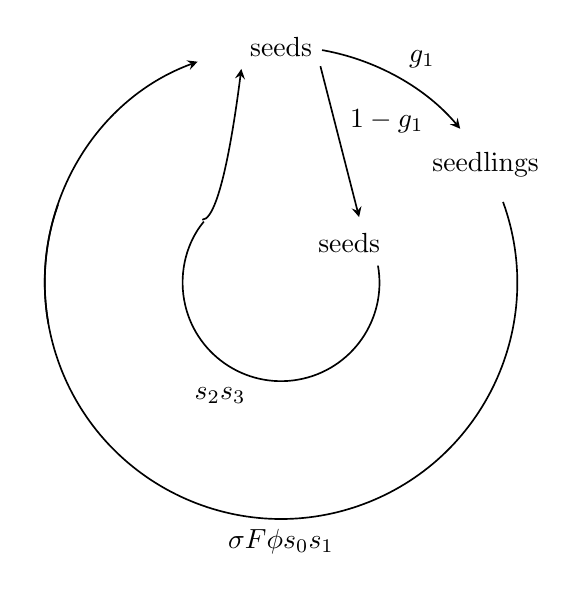
\begin{tikzpicture}[
            > = stealth, % arrow head style
            shorten > = 1pt, % don't touch arrow head to node
            auto,
            node distance = 2.75cm, % distance between nodes
            semithick % line style
        ]

        \tikzstyle{every state}=[
            draw = none,
            thick,
            fill = white,
            minimum size = 4mm
        ]
   
    \node (i) at (90:3cm)  {seeds};
   \node (j) at (30:3cm) {seedlings};
%   \node (k) at (210:3cm) {$k$};
   \node (h) at (30:1cm) {seeds};
%   \node (m) at (210:1cm) {seeds};
  % \node (n) at (30:1cm) {seeds};

   \draw[->] (80:3cm)  arc (80:40:3cm) node[midway]{$g_1$};
   \draw (20:3cm) arc (20:-200:3cm) node[midway]{$\sigma F \phi s_0 s_1$};
   \draw[->] (190:3cm) arc (190:110:3cm);

   \draw (10:1.25cm)  arc (10:-220:1.25cm) node[midway]{$s_2 s_3$};
    \draw[->] (.5,2.75) -- (1,.8) node[midway]{$1-g_1$};
    \draw[->] (-1,.8) parabola (-.5,2.75);

       
  \end{tikzpicture}
  \caption{Life cycle diagram for \textit{Clarkia xantiana}. \hl{I would like to draw a better life cycle diagram.}}\label{lifecycle}
 \label{fig:lifecycle}
\end{figure}


\begin{figure}[!htbp]
\centering
\begin{tikzpicture}[
            > = stealth, % arrow head style
            shorten > = 1pt, % don't touch arrow head to node
            auto,
            node distance = 2.75cm, % distance between nodes
            semithick % line style
        ]

        \tikzstyle{every state}=[
            draw = none,
            thick,
            fill = white,
            minimum size = 4mm
        ]

        \node[state] (Y1a) [] {$y^{\mathrm{tot}}_{ijt}$};
        \node[state] (Y1b) [right of=Y1a] {$y^{\mathrm{intact}}_{ijt}$};
        \node[state] (N) [left of=Y1a] {$n_{ijt}$};
        \node[state] (Y2) [right of=Y1b] {$y^{\mathrm{oct}}_{ijt}$};
        \node[state] (G) [below of=Y1b] {$y^{\mathrm{germ}}_{ijt}$};
     
        \node[draw] (O1) [above of=N] {$\mathrm{October}_{t-1}$};
        \node[draw,dotted] (J1) [above of=Y1a, align=center] {$\mathrm{January}_{t}$ \\ pre-germ};
        \node[draw,dotted] (J2) [above of=Y1b, align=center] {$\mathrm{January}_{t}$ \\ post-germ};
        \node[draw,fit=(J1) (J2)] {};
        \node[draw] (O2) [above of=Y2] {$\mathrm{October}_{t}$};

        \path[->] (N) edge node {$\theta_1$} (Y1a);
        \path[->,dotted] (Y1a) edge node {$$} (Y1b);
   	\path[->] (Y1b) edge node {$\theta_3$} (Y2);
       	\path[->] (Y1a) edge[bend right] node {$\theta_2$} (G);

        \node[state] (T1) [below right of=G] {$n^{\mathrm{gt}}_{ijt}$};
   	\path[dotted, ->] (Y2) edge node {} (T1);
        \node[state] (TG) [right of=T1] {$y^{\mathrm{gt}}_{ijt}$};
   	\path[->] (T1) edge node {$\theta_g$} (TG);
        \node[state] (T2) [below of=T1] {$n^{\mathrm{vt}}_{ijt}$};
   	\path[dotted, ->] (TG) edge node {} (T2);
        \node[state] (VG) [right of=T2] {$y^{\mathrm{vt}}_{ijt}$};
   	\path[->] (T2) edge node {$\theta_v$} (VG);
	
	\node[draw,fit=(N) (Y1a) (Y1b) (Y2) (G) , label={[label distance=0cm, align = right]left:{Seed bag \\ experiment}}] {};
	
	\node[draw,fit=(T1) (T2) (TG) (VG), label={[label distance=0cm, align = right]left:{Viability \\ trials}}] {};


  \end{tikzpicture}
  \caption{Diagram of data from the seed bag experiments and viability trials. There are two boxes: one for the seed bag experiment and one for the viability trials. In the seed bag experiment, I split January into two steps, one for just before germination and one for just after. Solid arrows represent probabilities estimated with a binomial experiment and are labeled with corresponding parameters. Dotted arrows represent cases where the seeds at the head of the arrow include some, possibly all, seeds at the tail of the arrow.}\label{seedexperiments}
 \label{fig:seedBagDiagram}
\end{figure}

\fi
\begin{figure}[h]
   \centering
       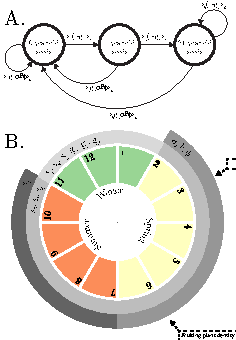
\includegraphics[scale=2]{../manuscript/figures/model-figure.pdf}  
        \caption{ Diagram representations of Clarkia life cycle. \hl{Note: Bottom panel needs to be edited so that the dotted lines on the outside of the figure are removed.} }
        \label{fig:life-cycle}
\end{figure}


\begin{figure}[!h]
       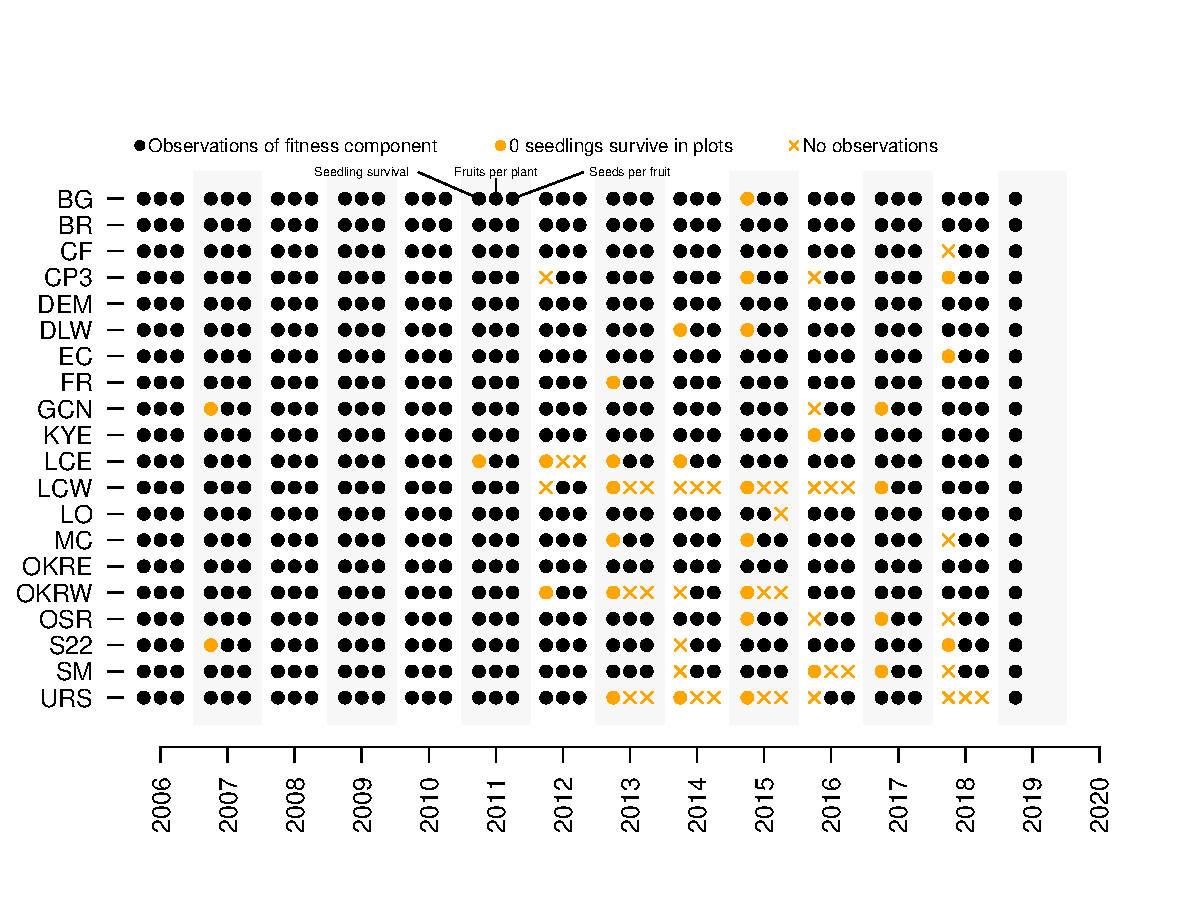
\includegraphics[width=\textwidth]{../figures/analysis/zero-fitness.pdf}  
    \caption{ Summary of the aboveground observations, low fitness, and no observations. }
 \label{fig:zero-fitness}
\end{figure}


\begin{figure}[!h]
       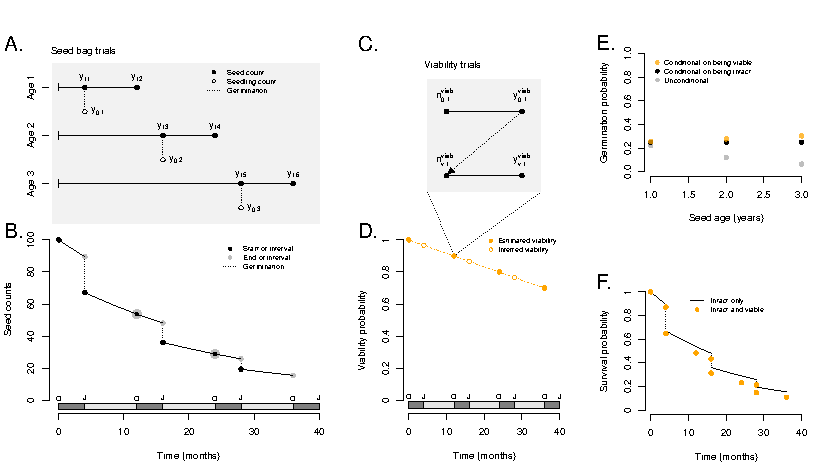
\includegraphics[width=\textwidth]{../manuscript/figures/seed-bag-figure.pdf}  
    \caption{ Summary of the seed bag burial experiments and viability trials. \hl{Figure will be labeled as (A-B: seed bag trials, C-D: viability trials, E-F: germination probability and survival probability. Add month markers to the y-axis in panels B, D, F}. (A) The gray panel contains a graphical representation of the seed bag trials. Seeds were buried at the start of each experiment (100 seeds in month 0). Seed bags were unearthed and intact seeds ($y_{\cdot \cdot}$) and germinants ($y_{\mathrm{g},\cdot}$ counted. The graph below the panel shows a hypothetical survival function associated with persistence of seeds in the soil seed bank. (B) The gray panel contains a graphical representation of the viability trials. Seeds were tested in two rounds; germination trials were performed and then some or all of the ungerminated seeds were tested for viability. The graph below the panel shows hypothetical data from a series of viability trials and the interpolated, inferred viabilities at times when viability was unobserved. (C) Age-specific germination probably is summarized in three ways. (D) The graph shows the survival function for persistence of seeds in the soil seed bank (black line) and the estimated discrete survival probabilities for persistence and viability of seeds (orange points). }
 \label{fig:seed-bag-experiments}
\end{figure}

\iffalse

 \begin{figure}[h]
   \centering
       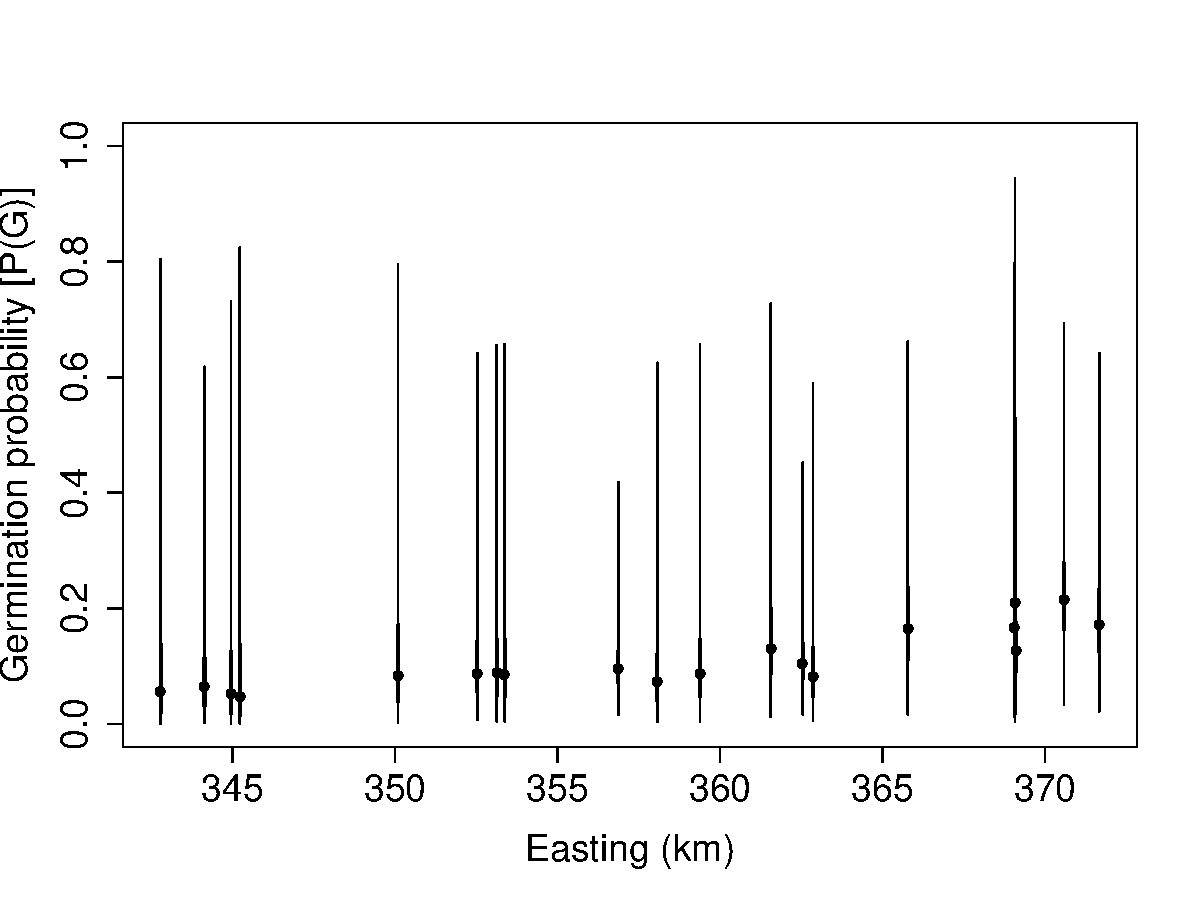
\includegraphics[page=1,width=1\textwidth]{../figures/spatial-g1.pdf}  
    \caption{ Germination probability plotted against easting (km). The plot shows the marginal posterior distribution for germination probability at each site. The points are the median of the posterior. The thinner line represents the 95\% credible interval and the thicker line represents the 50\% credible interval. }
 \label{fig:test}
\end{figure}

\fi

 \begin{figure}
\centering
\begin{subfigure}[h]{.65\textwidth}
\centering
       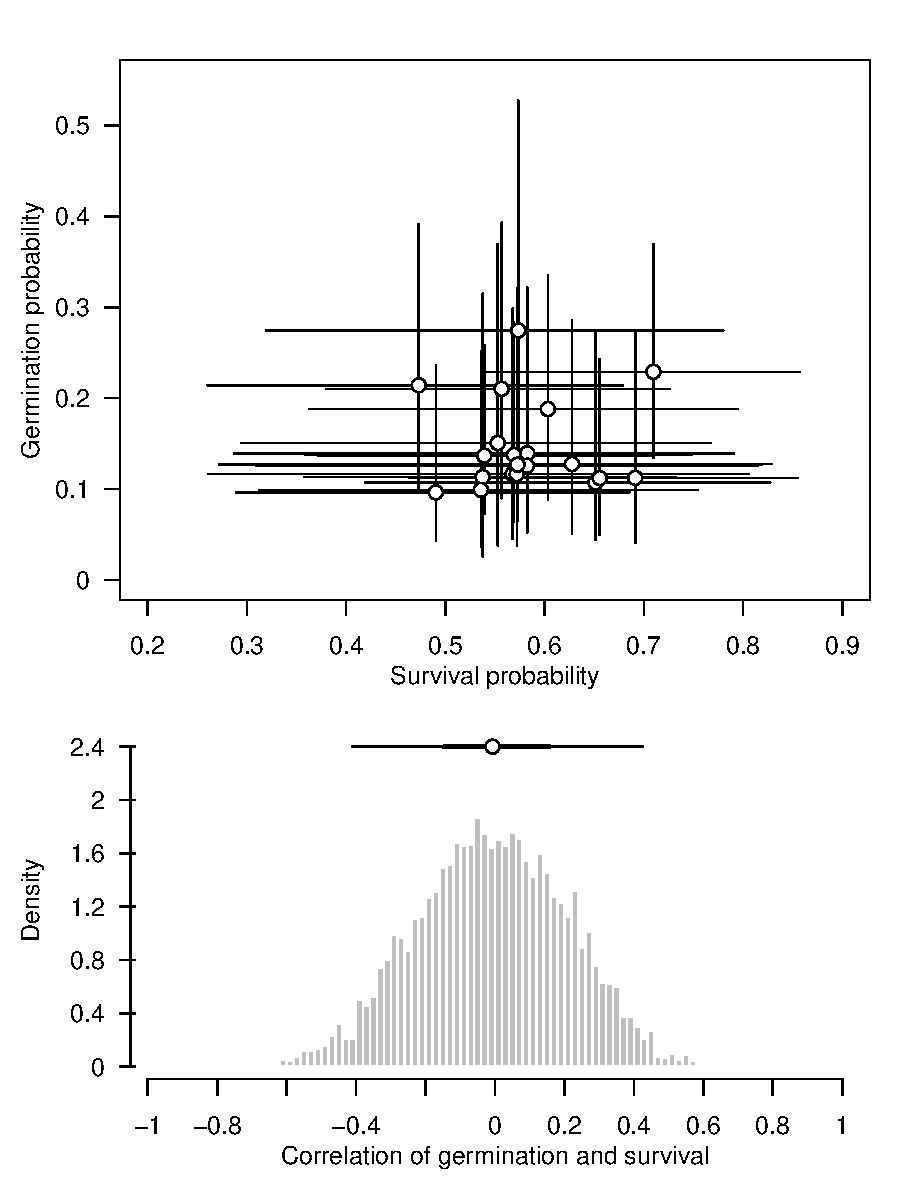
\includegraphics[page=1,width=1\textwidth]{../figures/analysis/correlation-germ-surv.pdf}  
\end{subfigure}
 \caption{ The top panel shows the observed germination probability plotted against probability of seed survival. The bottom panel shows the posterior distribution of correlation between observed germination probability and the probability of seed survival. }
  \label{fig:correlation-germ-surv}
 \end{figure}
 
 \begin{figure}
%\centering
%\begin{subfigure}[h]{.65\textwidth}
\centering
       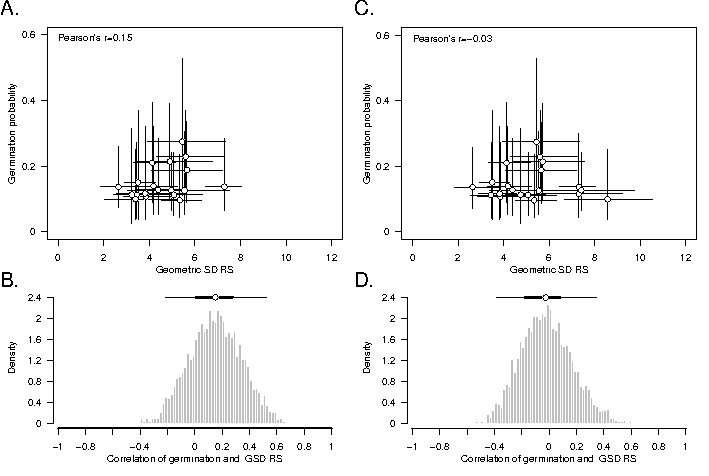
\includegraphics[page=1,width=1\textwidth]{../manuscript/figures/analysis-figure.pdf}  
%\end{subfigure}
%\begin{subfigure}[h]{.9\textwidth}
%\centering
%       \includegraphics[page=2,width=1\textwidth]{../figures/germ_rs_correlation.pdf}  
%\end{subfigure}
 \caption{ (A) The top left panel shows the observed germination probability plotted against the temporal variation in per capita reproductive success. (B) The bottom left panel shows the posterior distribution of correlation between observed germination probability and geometric SD of per capita reproductive success. (C) The top right panel shows observed germination probability plotted against the optimal germination probability predicted by a density-independent model. For each population, the observed germination probability is the obtained from the model for seed bank vital rates. Each point is the population-specific median of the posterior of $g_1$ for a model fit to data from seed bag experiments from 2006--2009. Data was pooled across years. The dotted line indicates a 1:1 relationship between observations and predictions. Values below the line indicate that the model predicts higher germination probabilities than observed; values above the line would indicate that the model predicts lower germination probabilities than observed. }
   \label{fig:obs-pred}
 \end{figure}
 
  \begin{figure}[h]
   \centering
  %#\begin{tabular}{@{}c@{\hspace{.5cm}}c@{}}
       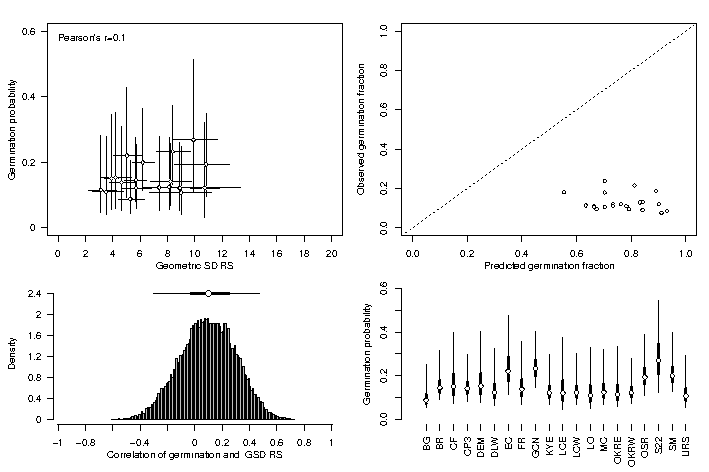
\includegraphics[page=1,width=.9\textwidth]{../manuscript/figures/analysis-figure-lowFitness.pdf}  
    \caption{ Results with low fitness years set to 0. (A) The top left panel shows the observed germination probability plotted against the temporal variation in per capita reproductive success. (B) The bottom left panel shows the posterior distribution of correlation between observed germination probability and geometric SD of per capita reproductive success. (C) The top right panel shows observed germination probability plotted against the optimal germination probability predicted by a density-independent model. For each population, the observed germination probability is the obtained from the model for seed bank vital rates. Each point is the population-specific median of the posterior of $g_1$ for a model fit to data from seed bag experiments from 2006--2009. Data was pooled across years. The dotted line indicates a 1:1 relationship between observations and predictions. Values below the line indicate that the model predicts higher germination probabilities than observed; values above the line would indicate that the model predicts lower germination probabilities than observed. }
 \label{fig:obs-pred-lowFitness}
\end{figure}

\clearpage
%%%%%%%%%%%%%%%%%%%%%%%%%%%%%%%%%%%%%%%%%%%%%%%%%%%%
% BIBLIOGRAPHY
%%%%%%%%%%%%%%%%%%%%%%%%%%%%%%%%%%%%%%%%%%%%%%%%%%%%
\bibliographystyle{/Users/gregor/Dropbox/bibliography/styleFiles/ecology} 
\bibliography{/Users/gregor/Dropbox/bibliography/seeds}

\clearpage
%%%%%%%%%%%%%%%%%%%%%%%%%%%%%%%%%%%%%%%%%%%%%%%%%%%%
% SUPPLEMENTARY MATERIAL
%%%%%%%%%%%%%%%%%%%%%%%%%%%%%%%%%%%%%%%%%%%%%%%%%%%%
\section*{Supplementary material}

%\subsection*{Theoretical background for hypotheses.} Explanation of key papers that develop theoretical results about seed banks. The document describes results from these papers that are relevant to understanding and interpreting the data in this manuscript. Link to document: \url{https://github.com/gregor-fausto/clarkiaSeedBanks/blob/master/products/appendices/appendix-cohen-results/appendix-x-cohen-results.pdf}

\subsection*{Data summary.} Summary tables for all datasets used in the manuscript. The document summarizes the types of data collected. The document provides a table summarizing each dataset (e.g. sample size per each site and year). Link to document: \url{https://github.com/gregor-fausto/clarkiaSeedBanks/blob/master/products/tables/data-summary.pdf}

\subsection*{Joint posterior.} Expression for the posterior proportional to the joint distribution, and corresponding directed acyclic graphs. Link to document: \url{https://github.com/gregor-fausto/clarkiaSeedBanks/blob/master/products/appendices/appendix-joint-posteriors/appendix-joint-posteriors.pdf}

\subsection*{Priors.} Explanation of priors. Link to document: \url{https://github.com/gregor-fausto/clarkiaSeedBanks/blob/master/products/appendices/appendix-priors/appendix-priors.pdf}

\subsection*{Model checks.} Model checks, including visual posterior predictive checks and assessments with Bayesian $p$-values for test statistics. Link to document: \url{https://github.com/gregor-fausto/clarkiaSeedBanks/blob/master/products/appendices/appendix-model-checks/appendix-x-model-checks.pdf}


%\subsection*{Data processing workflow.} Description of workflow for processing the data used in the analysis. The document describes how comma-separated value (.csv) and Excel (.xls and .xlsx) files were read and processed in R. Link to document: \url{https://github.com/gregor-fausto/clarkiaSeedBanks/blob/master/library/dataProcessingWorkflow.md}

%\subsection*{Method for estimating seed bank parameters using conditional probabilities.} The document explains how we compose conditional probabilities to calculate probabilities of survival and germination of seeds in the seed burial experiment. Link to document: \url{https://github.com/gregor-fausto/clarkiaSeedBanks/blob/master/products/appendices/appendix-conditional-probability/appendix-x-conditional-probability.pdf}


\end{document}